% 7-page submission cut of main.tex. Same numbers, same claims; evidence moved to the appendix.
% Generated alongside the full version; both compile from the same figures/ and refs.bib.
\documentclass[10pt]{article}
\usepackage[margin=0.75in]{geometry}
\usepackage{amsmath,amssymb,booktabs,enumitem,tabularx,array,graphicx,xcolor}
\usepackage{url}
\usepackage[numbers,sort&compress]{natbib}
\usepackage{placeins}
\usepackage{hyperref}
\hypersetup{colorlinks=true,allcolors=teal!50!black}
\setlength{\parskip}{0.25em}\setlength{\parindent}{0pt}
\newcommand{\gzero}{g{=}0}\newcommand{\DeltaAUROC}{\Delta\mathrm{AUROC}}

\title{\textbf{Auditing the Winner: Critic Disagreement Adds No Detectable\\ Failure Signal Beyond the Selector on SWE-Agent Trajectories}}
\author{Joseph Morante\\ \small Algoverse AI Research}
\date{\small September 2026}

\begin{document}\maketitle

\begin{abstract}
When an agent commits the best of $n$ attempts under a critic, the committed trajectory is where the critic's confidence and its errors coincide. A common proposal is to audit it with a disjoint panel of critics and escalate on disagreement. We pre-registered and ran this test with executed gold on SWE-bench Verified (41 instances, 9 repositories) and SWE-bench Multilingual (114 instances, 37 repositories): best-of-4 selection by a reward model, a checkpoint-disjoint panel, and the official test harness. Silent failures --- committed, agent-declared-complete trajectories that fail hidden tests --- were 35\% and 45\% of the population. On the registered endpoint, the out-of-fold gain in AUROC from adding panel disagreement to the selector's own score, disagreement adds nothing detectable: pooled over 47 failures and 46 repositories, the three estimators that use every row give $-0.03$, $-0.01$ and $+0.01$, every interval includes zero, and the loosest pooled upper bound is $+0.12$. Disagreement alone ranks failures at AUROC 0.51 and 0.57, indistinguishable from the selecting critic's own score, and this held across 4k--16k contexts, pruned overlapping windows, eight reward models from 1B to 32B, two re-selection regimes, and a single-family panel of LLM judges. Point estimates that cleared a structural baseline on the pilot all fell to chance on 37 repositories: no configuration produced a replicable signal. An unselected-candidate control shows that with this selector the committed candidate fails no more often than one passed over, while the selector's own score ranks failures at 0.81 among unselected candidates and 0.61 among committed ones --- the selection-conditional gap measured directly.
\end{abstract}

\section{Introduction}
Best-of-$n$ selection under a learned critic is a default in agent scaffolds: generate several trajectories, score each with a reward model, commit the argmax. Three claims about this are easy to conflate, and this paper keeps them apart. The \emph{theory} is that argmax selection on a noisy score induces the optimizer's curse~\citep{smith2006optimizer}: the top-scored candidate is disproportionately the one whose flaws the critic cannot see, so the score carries less information about the committed candidate than about the pool. What we \emph{observe} is one instance of that theory measured directly: on Verified the selecting critic ranks failures at 0.81 among candidates it passed over and 0.61 among those it committed, on the same instances. What we do \emph{not} show is that selection raised the failure rate of the committed candidate --- with the selector we used, it did not (\S\ref{sec:control}). A committed trajectory that fails while carrying a high score is a \emph{silent failure}; they are a third to a half of what this agent committed, whether or not selection put them there.

The obvious safeguard is a second opinion. If a panel of critics disjoint from the selector disagrees sharply about a committed trajectory, that disagreement might carry information the selector has exhausted. That correlated critics share blind spots is not our idea: the correlated-judge literature predicts it~\citep{goel2025great,kim2025correlated,kohli2026nine,hossain2026agreement,afrin2026ensembles}, and best-of-$n$ reward hacking is well characterised~\citep{gao2023scaling,khalaf2025inference,yu2026caution}. What had not been done is the measurement: put a disjoint panel on the population a critic actually committed, with executed gold, structural baselines and pre-registered bars, and ask what it adds over the selector. Our contributions:
\begin{itemize}[leftmargin=1.2em,itemsep=0pt]
\item \textbf{A selection-conditional evaluation protocol for audit signals} --- selected population, selector baseline, executed gold, pre-registered bars --- with its first two-benchmark instantiation on SWE-agent trajectories. Candidate-pool discrimination does not measure residual auditing value on the selected population~\citep{emadi2026scaling,trilemma2026}.
\item \textbf{A replicated null with an estimator-robust bound}: disagreement's incremental value is indistinguishable from zero under four estimators, loosest pooled upper bound $+0.12$ over 47 positives and 46 repositories.
\item \textbf{Diagnostics}: test--retest stability of long-window reward-model scores, the repository-clustering ceiling on effective $n$, and six instrument failures that each would have produced a false positive (appendix).
\end{itemize}
``Critic'' means an off-the-shelf reward model or LLM judge used without task-specific training. Trained trajectory verifiers~\citep{shum2025swerm,rahman2026scout,wang2026failfast} are a different class.

\section{Setup}
The unit is one committed trajectory. Gold $g\in\{0,1\}$ is trajectory-level success under the official \texttt{swebench} 5.x harness; the positive class is failure ($\gzero$). The selecting critic $c_{\mathrm{sel}}$ scores each of $n{=}4$ full candidates and commits the argmax; the audit panel $\{c_1,\ldots,c_m\}$ satisfies $c_{\mathrm{sel}}\notin\{c_i\}$ at checkpoint level, and $u$ is the sample standard deviation of their rank-normalised scores, with rank norms fit on training repositories only. The population is committed trajectories whose agent exited with a submission and a non-empty patch. M1 $=\mathrm{AUROC}(u)$, M2 $=\mathrm{AUROC}(-c)$, M3 $=$ M1 $-$ M2 with a repository-clustered bootstrap. Population, positive class, metrics, predictions and a stopping rule were committed to the repository before any gold existed; each later analysis was added as a dated amendment before its data existed.

\section{Silent failures are common; selection did not concentrate them}\label{sec:control}
\begin{figure}[t]\centering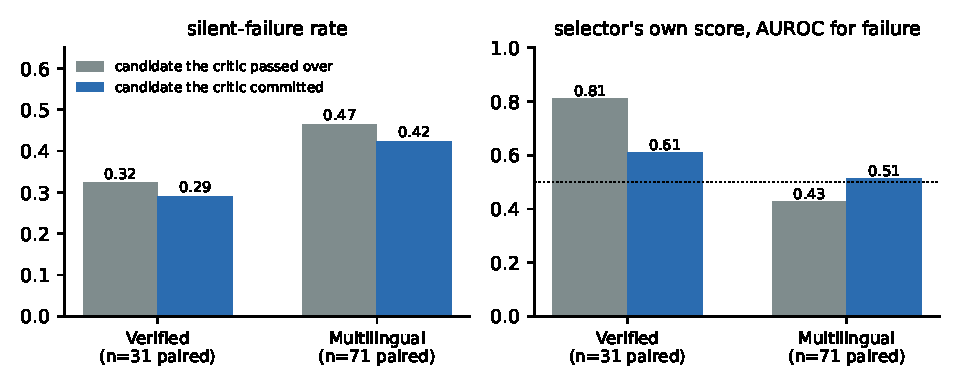
\includegraphics[width=0.92\linewidth]{figures/fig_control.pdf}
\caption{\textbf{Picking did not make things worse --- but it did use up the picker's own judgment.} One candidate the critic passed over, graded per instance, paired with the one it committed.}\label{fig:control}\end{figure}
Of 164 Verified candidates, 138 exited having submitted; selection by \texttt{Skywork-Reward-V2-Qwen3-4B} committed 34 usable trajectories, of which the harness resolved 22 and failed 12: \textbf{35.3\% [21.5, 52.1] silent failures}. On Multilingual the same pipeline gave 77 usable rows and 35 failures (45.5\%). Selection was real (the chosen index spread across all four slots) and $\mathrm{corr}(c,u)=0.11$.

Whether selection \emph{concentrated} failure is a separate question a committed-only sample cannot answer. Amendment 4f graded one unselected candidate per instance on both benchmarks (31 and 71 paired rows). \textbf{The committed candidate failed no more often than one passed over}: $-3$ points on Verified [$-21$, $0$] and $-4$ on Multilingual [$-11$, $+3$]. With this selector, best-of-4 did not concentrate failure, and we claim a failure \emph{rate}, not concentration. The control does measure the selection-conditional gap: on Verified the selector ranks failures among candidates it did not pick at 0.81 [0.74, 1.00] and among those it committed at 0.61 on the same instances. On Multilingual the critic has no signal in either arm (0.43, 0.51), so there was nothing to remove.

\section{Disagreement does not detect them}
The primary analysis --- four chat-preference reward models auditing a 4{,}096-token prefix --- gave $\mathrm{AUROC}(u)=0.508$ against the selector's own 0.621. Every amendment was declared before its data existed and asked whether some limitation of the primary was hiding a signal: scoring the final diff plus the last 3k tokens ($u=0.458$); six chat RMs from 1B to 8B with the patch in view (panel 0.494); re-selecting with the proposal's named 8B critic ($u=0.455$) and with a code-trained model ($u=0.542$); a true 16k context (panel 0.439); \texttt{AceCodeRM-7B} (0.405 as a detector) and its 32B sibling (0.557); and three LLM judges, where \texttt{gpt-5} reached 0.720 and \texttt{gpt-5-mini} 0.752 individually but their disagreement was 0.528. Every registered prediction that panel disagreement carries signal beyond the selector failed (Table~\ref{tab:ladder}). One registered bar was cleared and we disclose it rather than report only the failures: the primary hypothesis was registered as the bare inequality $\mathrm{AUROC}(u) > 0.5$, and $u$ is 0.508 and 0.565, so it passes as written. We do not treat it as a detector, because the bar carries no minimum effect size, both intervals include chance, and the paired comparisons against the selector are $-0.114$ and $+0.005$. Registering a threshold with no margin was our design error; overruling it is post hoc and labelled so. Other registered predictions that passed are reported where they arise: the premise check on the silent-failure rate, the single-detector bar for the best LLM judge, the three bars of the windowed amendment below, and the replication's own prediction that the null would hold. One registered prediction, on the code-trained critic's prefix-versus-full-length score correlation, is not evaluable because that model fell back to a 4k window on 31 of 34 rows; we report it as attempted and undecidable.
\begin{table}[t]\centering\footnotesize
\begin{tabular}{lcccc}\toprule
Configuration & $\mathrm{AUROC}(u)$ & $\mathrm{AUROC}(-c)$ & M3 & 95\% CI \\\midrule
Primary: 4k prefix, 4 chat RMs & 0.508 & 0.621 & $-0.114$ & $[-0.37, +0.22]$ \\
\quad robustness, $m{=}3$ family-disjoint & 0.545 & 0.621 & $-0.076$ & $[-0.39, +0.23]$ \\
Submission window: diff + last 3k tok & 0.458 & 0.530 & $-0.072$ & $[-0.35, +0.13]$ \\
Patch in view (4k), 4 chat RMs & 0.494 & 0.621 & $-0.127$ & $[-0.28, +0.11]$ \\
\quad + AceCodeRM-7B as 5th auditor & 0.473 & 0.621 & $-0.148$ & $[-0.30, +0.10]$ \\
8B named critic selecting; disjoint panel & 0.455 & 0.602 & $-0.148$ & $[-0.49, +0.26]$ \\
\quad the same at a true 16k (33 rows) & 0.483 & 0.736 & $-0.252$ & $[-0.47, +0.28]$ \\
Code-trained critic selecting; 5-RM panel & 0.542 & 0.472 & $+0.069$ & $[-0.21, +0.45]$ \\
Full trajectory, true 16k, 4 chat RMs & 0.439 & 0.621 & $-0.182$ & $[-0.38, +0.17]$ \\
LLM judges (gpt-5 family), patch in view & 0.528 & 0.621 & $-0.093$ & $[-0.30, +0.10]$ \\
\quad execution-aware (+ last 6k tok) & 0.640 & 0.621 & $+0.019$ & $[-0.28, +0.16]$ \\\midrule
Pruned overlapping windows, $u_{\max}$ & \textbf{0.686} & 0.621 & $+0.064$ & $[-0.11, +0.33]$ \\\bottomrule
\end{tabular}
\caption{Every pre-registered configuration on the pilot. Same 34 trajectories and 12 positives, except the re-selection rows (12, 11 and 11). M3 $=$ M1 $-$ M2; repository-clustered bootstraps on the paired difference. Only the last row crosses the structural baseline of 0.665, and it did not replicate (\S\ref{sec:replication}).}\label{tab:ladder}\end{table}

One configuration crossed its bar. Amendment 3 pruned tool outputs and scored overlapping 3{,}500-token windows, taking the panel's maximum disagreement: $\mathrm{AUROC}(u_{\max})=0.686$ against a pre-registered bar of 0.665, with a free permutation $p=0.04$ that rises to $p=0.21$ within repository and a leave-one-instance-out range of 0.657--0.731 that straddles the bar.

\section{Replication on 37 repositories}\label{sec:replication}
\begin{figure}[t]\centering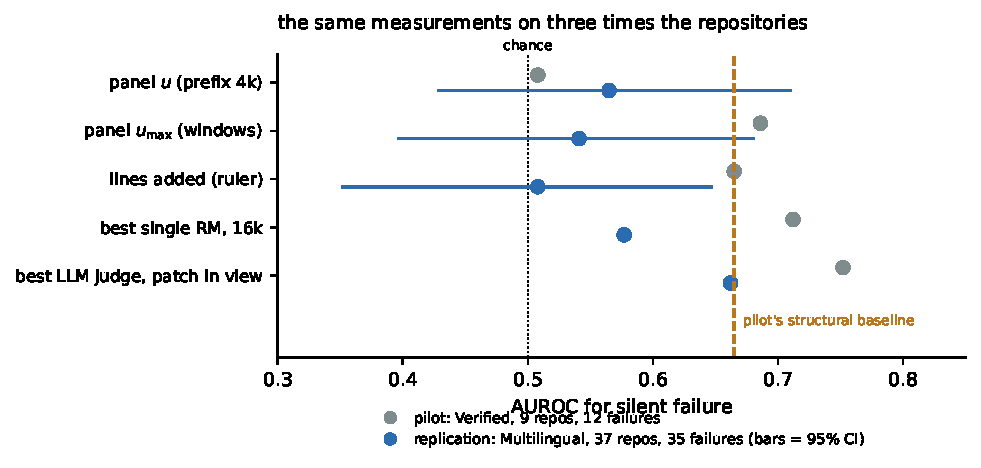
\includegraphics[width=0.92\linewidth]{figures/fig_replication.pdf}
\caption{\textbf{Everything promising on the small benchmark vanished on the big one.}}\label{fig:replication}\end{figure}
The binding limitation of the pilot is nine repositories. Amendment 4e, pre-registered before any trajectory existed, re-ran the instrument on SWE-bench Multilingual: 41 repositories in nine languages (37 survive into the analysed population), 114 instances, 456 trajectories, the same selector and panel, agent sandboxes and gold on Modal, with three reference-patch / empty-patch oracle pairs passed before any model patch was graded.

\textbf{R-P1} (the null replicates): panel $u$ 0.565 [0.43, 0.71] against the critic's 0.560; paired difference $+0.005$ [$-0.19$, $+0.22$]; within-repository permutation $p=0.85$. \emph{Passed.} \textbf{R-P2} (the windowed positive confirms): $u_{\max}$ 0.541 [0.40, 0.68], within-repository $p=0.53$, leave-one-out 0.528--0.557. \emph{Failed.} \textbf{R-P3} is vacuous: $u_{\max}$ exceeds the lines-added baseline only because that baseline itself fell from 0.665 to 0.508 [0.35, 0.65]. Patch size predicted silent failure on Verified and does not here. The best reward model at 16k is 0.577 (the 1B model that scored 0.712 is at 0.485); the named 8B critic 0.52; the code-trained model 0.356; LLM judges 0.58--0.66 with disagreement 0.514.

\section{The registered endpoint}\label{sec:endpoint}
\begin{table}[t]\centering\footnotesize
\begin{tabular}{llcccc}\toprule
Estimator & Population & base & $+u$ & $\DeltaAUROC$ & 95\% CI \\\midrule
Logistic, leave-one-repo-out (pre-registered) & Pooled & 0.484 & 0.454 & $-0.030$ & $[-0.10, +0.04]$ \\
Logistic, 5 clustered folds & Pooled & 0.504 & 0.491 & $-0.014$ & $[-0.09, +0.07]$ \\
AUROC within fold, size-weighted & Pooled & --- & --- & $-0.119$ & $[-0.31, +0.28]$ \\
Fixed unit weights, no fitting & \textbf{Pooled} & \textbf{0.559} & \textbf{0.571} & $\mathbf{+0.013}$ & $\mathbf{[-0.07, +0.12]}$ \\\bottomrule
\end{tabular}
\caption{The registered confirmatory endpoint under four estimators, 111 rows, 47 positives, repository-clustered bootstrap. The last three are post-hoc robustness checks of the first. The within-fold estimator drops repositories where no AUROC is defined and covers 53 of 111 rows. Per-benchmark rows are in the appendix.}\label{tab:endpoint}\end{table}
The proposal's confirmatory quantity was the held-out $\DeltaAUROC$ of $M_{c+u}$ over $M_c$. The 70/30 repository split never held ten test positives, so it was never eligible on the pilot alone; with 47 positives across both benchmarks it can be computed by leave-one-repository-out, a declared substitution of the cross-validation scheme, not of the estimand. Because a two-parameter model refit on eight to thirty-six clusters is fragile, we compute it four ways (Table~\ref{tab:endpoint}). They disagree in sign. They agree on the conclusion: every interval includes zero, and among the three estimators that use every row the loosest pooled upper bound is $+0.12$ ($+0.25$ on the pilot alone). The fixed-weight variant reproduces the raw $\mathrm{AUROC}(-c)$ almost exactly (0.559 vs.\ 0.560) while the logistic variants report $M_c$ at 0.48--0.50: pooling out-of-fold probabilities across folds with different intercepts scrambles the global ranking, depressing both arms and largely cancelling in the difference. With rank metrics and few clusters this can make a real signal appear to vanish; an unfitted combination is the cheap check.

\section{A capable selector, and newer judges}\label{sec:selector}
Amendment 5 re-scored every candidate in both pools with \texttt{gpt-5} and committed its argmax (620 candidates, \$13, 59 new patches graded). A defect found in review must be stated first: the analysis filtered its population by the \emph{4B}-committed candidate's agent-declared-complete flag rather than the \texttt{gpt-5}-committed one, which on Multilingual dropped 16 eligible instances. Verified is unaffected; the corrected Multilingual set is 101 rows and 44 failures, and the numbers below are the corrected ones.

S-P1 passes on both registered conditions: pool $\mathrm{AUROC}(-c)$ of 0.712 and 0.706, and a committed failure rate below the random arm's, paired within instance, at $-0.065$ [$-0.20$, $0.00$] and $-0.084$ [$-0.14$, $-0.03$], with no pair where the committed trajectory failed and the random one passed. S-P2 fails on both: the gap is $-0.080$ on Verified and 0.035 on Multilingual against a registered bar of 0.10, so we withdraw the claim that selection measurably consumes a strong selector's signal and keep only the 4B observation on Verified (0.81 to 0.61). S-P3 fails on its first condition, $\mathrm{AUROC}(u) = 0.591$ against a bar of 0.60, and the endpoint agrees across estimators for the first time in this study: $+0.012$, $-0.024$, and $-0.018$ [$-0.11$, $+0.07$] unfitted. The defect also explains the study's most alarming number: the registered logistic's $+0.375$ [$+0.21$, $+0.52$], with a baseline collapsed to 0.150, becomes $+0.012$ with a baseline of 0.575. That cell is \emph{consistent with} the null and does not establish it, since the upper bound of $+0.073$ exceeds the $+0.05$ we declared actionable.

Newer judges sharpen the dissociation rather than resolving it. \texttt{gpt-6-sol} reaches 0.776 [0.68, 0.87], the best single detector in the study, and both \texttt{gpt-6} judges beat every \texttt{gpt-5} judge on both benchmarks, while the newer pair's disagreement falls to 0.41 against the weaker trio's 0.51 and a five-judge panel gives 0.44 [0.31, 0.58]. Better critics, no better disagreement. Exploratory, one vendor, and a two-member spread is a weaker statistic than a four-member one.

\section{Mechanism: stable critics, uninformative disagreement}
Re-scoring an identical window after a content-preserving reformatting, every critic reproduces its ranking at $r=0.98$--$0.99$; after a 128-token shift, at $0.86$--$0.95$; the per-window panel $u$ at $0.91$ and $0.73$. Adjacent windows with 25\% overlap correlate at $0.20$--$0.56$, first against last at $-0.39$ to $0.47$. These critics are stable instruments responding to what is in front of them: the prefix score judges the problem, the patch score judges the patch, and they differ because the inputs do. An earlier draft read that difference as critic instability; this test withdraws that claim. The failure is in the statistic. A panel's disagreement is large when its members' rank-normalised scores spread out, and that spread is dominated by between-critic heterogeneity rather than by shared uncertainty about correctness: the signal individual critics carry (0.71--0.75 at length on the pilot) is averaged away, not amplified.

\section{The instrument, and seven ways it lied to us}
Each of the following produced a plausible result that was wrong, and each was caught by an oracle control or a regression test rather than by inspecting the numbers. (1) A sandbox flag hid \texttt{numpy} from the gold harness: every trajectory scored as a failure; caught because the benchmark's reference solutions are run through the harness before any model patch. (2) An LLM-as-judge selecting critic emitted three distinct values over 640 candidates, so best-of-16 silently became first-draw and 39 of 40 committed trajectories were identical to the $n{=}4$ run; caught by the chosen-index histogram. (3) On a fresh VM the harness's image pulls failed on an architecture manifest: 41/41 failures in 499 seconds; caught by the harness's own error count. (4) Our power function reported $\approx$0.40 ``power'' under the true null; caught by simulating the null. (5) Repository grouping truncated hyphenated names, corrupting the held-out split. (6) Rank normalisation was fit on all rows, leaking test rows into the panel statistic; every $u$ reported here is post-fix, verified by recomputing the stored values from raw panel scores with training-repository normalisation (max absolute difference $0.0$). (7) The selector-axis analysis filtered its population by the previous selector's committed candidate rather than the new one's, dropping 16 eligible instances and manufacturing a $+0.375$ gain from a collapsed baseline; on the correct population it is $+0.012$ (\S\ref{sec:selector}). The rule we adopted: a rate of exactly 0\% or 100\%, or a statistic that cannot move, is an instrument, not a result. We report these because the same failure modes would let a positive result through unexamined.

\section{Limitations}
\begin{itemize}[leftmargin=1.2em,itemsep=0pt]
\item \textbf{One agent; two selectors, both off the shelf.} gpt-5-mini at 40 steps throughout. The primary selector is a 4B chat reward model, so the primary selected population is that of a weak selector; \S\ref{sec:selector} re-selects with \texttt{gpt-5}. Neither is a deployed-grade trajectory verifier. A stronger \emph{agent} is the open axis.
\item \textbf{The selection-conditional regime is observed on one benchmark.} On Multilingual the selector had no signal in either arm, so ``residual value after the selector has consumed its signal'' is measured only on the pilot. The replication settles the null for disagreement; it does not by itself place the study in the regime the proposal named. A selector that ranks failures in the pool was the missing experiment; Amendment 5 ran it (\S\ref{sec:selector}) and enters the regime on Multilingual, where the verdict is inconclusive rather than null.
\item \textbf{Critic classes.} Six chat-preference RMs, two code-trained RMs, five LLM judges from one vendor across two generations. Cross-vendor judges and trained trajectory verifiers were not run; the claim is scoped to off-the-shelf critics.
\item \textbf{Gold is the harness verdict}, which accepts some incorrect patches and rejects some correct ones~\citep{wang2025solved,rajan2026auditing,agentlens2026}; failure rates are lower bounds and AUROCs attenuated. Bounding the lucky-pass direction: no passing trajectory edited a test file, 4 of 64 passes are disjoint from the reference patch, and dropping or relabelling those four moves the pooled endpoint to $-0.053$ and $-0.024$ --- further from the safeguard working, not towards it.
\item \textbf{Forty-seven positives.} Intervals are $\pm0.25$ (pilot) and $\pm0.14$ (replication). Roughly twenty-five analyses were run on the twelve pilot positives without multiplicity correction; the replication is the correction. The study supports failure to reject and an upper bound, not equivalence to chance.
\item \textbf{Repository clustering.} Verified is 500 instances over 12 repositories (django 46\%); the public ICC of resolution by repository is 0.033--0.053, an effective $n$ of 64--95 of 500. The paired ``beat the baseline by 0.10'' test has power $\approx$0.3 at any $n$, which is why the replication changed repositories rather than instances.
\item \textbf{Exploratory analyses.} The diversity-versus-error-correlation experiment was run after the confirmatory results: no decorrelated panel exists among these critics, all 35 four-member panels sitting at pairwise error correlation 0.71--0.89, and within that range correlation does not predict performance. Judge calibration, a test-derived failure taxonomy, and a lucky-pass contamination bound were likewise post hoc and carry no multiplicity correction. Deviations, including a generation cap exceeded by \$3.30 and a registered difficulty control replaced after it proved to be a near-oracle, are listed in the appendix.
\end{itemize}

\section{Related work}
Selecting the argmax of a learned proxy over-optimises it~\citep{gao2023scaling,beirami2024theoretical}; at inference time this is reward hacking growing with $n$~\citep{khalaf2025inference,stroebl2024inference,brown2024monkeys}, mitigable by pessimism~\citep{yu2026caution}; the statistical form is the optimizer's curse~\citep{smith2006optimizer} and structural selection bias~\citep{hernan2004structural}. Two recent notes make the evaluation consequence explicit: success counted before an answer is chosen is not deployed success~\citep{emadi2026scaling}, and best-of-$n$ degrades calibration even under a perfect ranker~\citep{trilemma2026}. Ensembles mitigate but do not eliminate over-optimisation~\citep{eisenstein2023helping,coste2023reward}; uncertainty-aware and calibrated reward models change \emph{selection}~\citep{lou2024urm,park2025calibration}. Capable models make correlated errors~\citep{goel2025great,kim2025correlated}, judge panels supply few effective votes~\citep{kohli2026nine,hossain2026agreement}, common-mode error is not identifiable from internal scores~\citep{afrin2026ensembles}, and on code, verification helps only on margin-pivotal cases~\citep{shu2026pivotal,shu2026unanimity}. Process and generative verifiers score and select~\citep{lightman2023verify,wang2024mathshepherd,zhang2024genrm,xi2025agentprm}. Our testbed is SWE-bench and its subsets~\citep{jimenez2024swebench,swebenchverified2024,yang2025multilingual} with mini-SWE-agent~\citep{miniswe2025}; execution-free SWE critics~\citep{yadavally2025critics,shum2025swerm} and trained failure locators~\citep{rahman2026scout,wang2026failfast,sadhuka2025evaluator} target failure directly, but none conditions on an upstream selector. Agents declare success falsely~\citep{advani2026silent} and are overconfident~\citep{kaddour2026agentic}. Reward models used: \citep{liu2025skywork2,yang2024grm,zeng2025acecoder}, chosen by RewardBench standing~\citep{lambert2024rewardbench,malik2025rewardbench2}. On method, paired AUROC comparison for nested models should not use DeLong~\citep{demler2012misuse,pepe2013testing}; we follow clustered ROC practice~\citep{obuchowski1997nonparametric} and the registered-report tradition~\citep{nosek2018preregistration,chambers2022registered}.

\section{Conclusion}
A third to a half of what a reward-model critic confidently committed on two SWE benchmarks was broken. Disagreement among a disjoint panel of off-the-shelf critics did not yield a replicable failure-detection signal under any configuration we pre-registered and ran. One configuration crossed its bar on the pilot --- maximum disagreement over pruned windows, 0.686 on twelve positives --- and did not survive replication. The critics are not the problem: they are stable, content-driven, and given the solution at length a frontier judge ranks silent failures at about two-thirds. What fails is the idea that their \emph{disagreement} is where the missing information lives. Anyone building an escalation trigger for critic-selected agents should evaluate it where it will be used --- on the selected population, against the selector's own score, with executed gold --- and should expect off-the-shelf disagreement to add at most $+0.12$ AUROC \emph{beyond the selector's own score} --- which is the comparison that matters, since the selector's score is already in hand.

{\small\textbf{Reproducibility.} Code, pre-registrations with every dated amendment, every scored row, every critic's scores, the harness reports and a research log are in the repository. All figures regenerate from committed JSON. The extended version of this paper contains the full configuration ladder, the replication table, window and stability diagnostics, operating points, the instrument record and the chronology.}

\bibliographystyle{plainnat}
\bibliography{refs}
\end{document}
